\section{Simplicial Homotopy}

Aim: Introduce the notion of homotopy between maps of simplicial sets.

\begin{defi}
    Let $f,g \colon K \to X$ be morphisms of simplicial sets
\end{defi}

A homotopy $h\colon f \to g$ is a morphism $\Delta^1 \times K \xrightarrow{h} X$ such that 
\[
\begin{tikzcd}
    \Delta^{\{0\}} \times K \cong K
    \ar[d, "i_0 \times \id"']
    \ar[dr, "f"]
    \\
    \Delta^1 \times K 
    \ar[r,"h"]
    &
    X
    \\
    \Delta^{\{1\}}\times K \cong K
    \ar[u,"i_1 \times \id"]
    \ar[ur, "g"']
\end{tikzcd}
\]

\begin{exmp}
    Let $x,y \colon \Delta^0 \to X$ be vertices of $X$. 
    A homotopy $h\colon x \to y$ is a map $h$ such that
    \[
    \begin{tikzcd}
        \Delta^{\{0\}} \times K \cong K
        \ar[d, "i_0 \times \id"']
        \ar[dr, "x"]
        \\
        \Delta^1 \times K 
        \ar[r,"h"]
        &
        X
        \\
        \Delta^{\{1\}}\times K \cong K
        \ar[u,"i_1 \times \id"]
        \ar[ur, "y"']
    \end{tikzcd}
    \]
    that is $h \in X_1$ such that $d_1(h)=x$ and $d_0(h)=y$.
\end{exmp}

\subsection{Adjoint description of homotopy}
Let $f,g \in \Hom(K,X) = \underline{\Hom}(K,X)_0$ and $h\colon f\mapsto g$, that is $h \in \Hom(\Delta^1 \times K, X) = \underline{\Hom}(K,X)_1$ such that $d_1(h)=f$ and $d_0(h)=g$.

\underline{Upshot} Homotopy of maps $K \to X$ is an equivalence relation if $\underline{\Hom}(K,X)$ is a Kan complex.
So take the following lifting problem

\[
    \begin{tikzcd}
        \Lambda_k^n
        \ar[r,"\sigma"]
        \ar[d,"\iota"]
        &
        \underline{\Hom(K,X)}
        \ar[d]
        \\
        \Delta^n
        \ar[ur, dashed, "\exists"]
        \ar[r]
        &
        \Delta^0
    \end{tikzcd}
\]
which equates to the following lifting problem due to the adjunction of the inner hom and the product.
\[
\begin{tikzcd}
    \Lambda^n_k \times K
    \ar[r, " \overline{\sigma} "]
    \ar[d, " i \times \id_K"' ]
    &
    X
    \\
    \Delta^n \times K
    \ar[ru, dashed, " \overline{ \rho }"']
\end{tikzcd}
\]
If now $X$ were a Kan complex, then we would obtain a lift if $ i \times \id_K $ is an anodyne extension.

\begin{defi}
    Let $i\colon L \hookrightarrow K$ is a monomorphism in $\SetD$.
    Let $f,g \colon K \to X$ be such that $f \circ i = g \circ i$ we also write $(f_{\mid L}=g_{\mid L})$. A homotopy $h\colon f \to g $ (rel $L$) is a homtopy $h \colon f \to g$ such that 
    \[
    \begin{tikzcd}
        \Delta^1 \times L 
        \ar[r, "\pi_L"]
        \ar[dr,"1_{\alpha}"]
        \ar[d, "\id \times i"']
        &
        L
        \ar[d, "f_{\mid L} = \alpha = g_{\mid L}"]
        \\
        \Delta^1 \times K 
        \ar[r, "h"]
        &
        X
    \end{tikzcd}
    \]
    where $1_{\alpha}$ is given by $\Delta^1 \times L \xrightarrow{(!,\id_L)} \Delta^0 \times L \xrightarrow{\alpha}X$ and $!$ is the unique map into the terminal object.
\end{defi}

\subsection{Adjoint description of relative homotopy}

Consider the pullbackdiagram

\[
\begin{tikzcd}
    \Delta^1
    \ar[rd,"\Tilde{h}"]
    \ar[rrd,bend left,"h"]
    \ar[ddr, bend right]
    \\
    &
    \underline{\Hom}(K,X)_{\alpha}
    \ar[r]
    \ar[d]
    &
    \underline{\Hom}(K,X)
    \ar[d,"i^*"]
    \\
    &
    \Delta^0
    \ar[r,"\alpha"]
    &
    \underline{\Hom}(L,X)
\end{tikzcd}
\]

A morphism $\overline{h}$ into the fiber induces a homotopy $ h $ that is constant on $L$, thus this pullback gives us the construction of homotopy relative the simplical subset $L$.

We want that given a Kan complex $X$, to get that $ \underline{\Hom} ( K , X ) \xrightarrow{i^*} \underline{\Hom} ( L , X ) $ is a Kan fibration and finally get that $ \underline{ \Hom } ( K , X )_{\alpha} $ is a Kan complex and that homotopy ( rel $L$ ) is the equivalence relation on vertices of $ \underline{ \Hom } ( K , X )_{\alpha}$.

Rest is for now omitted since I cannot read my own notes.
Lecture 10.12

\begin{prop}
    The following classes have the same saturated closure
     \[
     \begin{tabular}{c}
          $B_1\coloneqq \{\Lambda_k^n \hookrightarrow\Delta^n \mid 0\leq n,0 \leq k \leq n \}$
          \\
          $B_2\coloneqq \{(\Delta^1 \times \partial \Delta^n) \cup(\Delta^{\{l\}} \times \Delta^n) \xhookrightarrow{i} \Delta^1 \times \Delta^n \mid 0 \leq n, l \in \{0,1\}\}$
          \\
          $B_3 \coloneqq
          \{ ( \Delta^1 \times L) \cup(\Delta^{\{0\}} \times K) \hookrightarrow \Delta^1 \times K \mid L \subseteq K \}$
     \end{tabular}
     \]
     where the product $\Delta^1 \times \Delta^n = N ( [1]) \times N([n]) \cong N ( [1] \times [n] )$ and $[1] \times [n] $ is given by the following diagram:
     \[
     \begin{tikzcd}
         00
         \ar[r]
         \ar[d]
         &
         01
         \ar[r]
         \ar[d]
         &
         \dotsc
         \ar[r]
         &
         0n
         \ar[d]
         \\
         10 
         \ar[r]
         &
         11
         \ar[r]
         &
         \dotsc
         \ar[r]
         &
         1n
     \end{tikzcd}
     \]
\end{prop}

As an example for $l=1$ and $n=2$ the domain of a morphism in $B_2$ is given by the following diagram, where the red triangle indicates 2-simplex with its interior removed.
\[
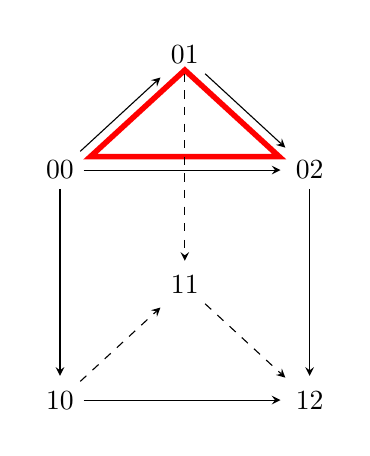
\begin{tikzpicture}[>=stealth,->,shorten >=2pt,looseness=.5,auto]
            \matrix[anchor=center, column sep=1cm, row sep=1cm] at (0,0)
            {
                                & \node(01) {$01$};   &                 \\
             \node(00) {$00$};     &                  & \node(02) {$02$}; \\
                                & \node(11) {$11$};   &                  \\
            \node(10) {$10$};    &                     & \node(12) {$12$}; \\ 
            };
            \draw[line width=2pt,color=red] (-1.2,0.9) -- (1.2,0.9) -- (0, 2) -- cycle;
            \begin{scope}[every node/.style={font=\small\itshape}]
                \draw (00) --  (01);
                \draw (00) --  (02);
                \draw (01) --  (02);
                \draw (00) --  (10);
                \draw [dashed] (01) --  (11);
                \draw (02) --  (12);
                \draw [dashed]  (10) --  (11);
                \draw   (10) --  (12);
                \draw [dashed]   (11) -- (12);
            \end{scope}
    \end{tikzpicture}
\]

\begin{proof}
    Note that 
    $\overline{\{\partial \Delta^n \hookrightarrow \Delta^n \mid n \leq 0 \}}$
    is given by the monomorphisms.
    ($\overline{B_2} \subseteq \overline{B_1}$) 
    We exhibit $i$ as a finite composition of anodyne extensions
    
    Let $(\Delta^1 \times \Delta^n)^{(-1)} \coloneqq(\Delta^1 \times \partial \Delta^n) \cup ( \Delta^{l} \times \Delta^n)$ and $(\Delta^1 \times \Delta)^{(n)} \coloneqq\Delta^1 \times \Delta^n$ so that we obtain the following coposition of morphisms.
    \[
    \begin{tikzcd}
        (\Delta^1 \times \Delta^n)^{(-1)} \hookrightarrow (\Delta^1 \times \Delta^n)^{(0)} \hookrightarrow (\Delta^1 \times \Delta^n)^{(1)}\hookrightarrow \dotsc \hookrightarrow(\Delta^1 \times \Delta^n)^{(n)} 
    \end{tikzcd}
    \]
    The non-degenerate (n+1)-simplices in $\Delta^1 \times \Delta^n$ are chains of the form
    \[
    \begin{tikzcd}
        00
        \ar[r]
        &
        01
        \ar[r]
        &
        02
        \ar[r]
        &
        \dotsc
        \ar[r]
        &
        0k
        \ar[d]
        \\
        &&&&
        1k
        \ar[r]
        &
        1(k+1)
        \ar[r]
        &
        \cdots
        \ar[r]
        &
        1n
    \end{tikzcd}
    \]
    for $0 \leq k \leq n$.
    We have that $(\Delta^1 \times \Delta^n)^{(i)} \subseteq \Delta^1 \times \Delta^n$ is the smallest subset containing $( \Delta^1 \times \partial \Delta^1)^{(-1)}$ and the non degenerate $(n+1)$ simplices $h_j$ for $0 \leq j \leq i$.
    Which means it is given by the following pushout square
    \[
    \begin{tikzcd}
        \Lambda_{i+1}^{n+1}
        \ar[r]
        \ar[d, hook, " B_1 \ni"']
        &
        (\Delta^1 \times \Delta^n)^{(i-1)}
        \ar[d, hook, "\in \overline{B}_1"]
        \\
        \Delta^{n+1} 
        \ar[r, "h_i"]
        &
        (\Delta^1 \times \Delta^n)^{(i)}
    \end{tikzcd}
    \]

        
    Let us take a look at the example for the case $n=2$ in detail.
    We iteratively add 3-simplices into $\partial \Delta^2 \times \Delta^1 \cup \Delta^2 \times \Delta^1$.
    \[
    \begin{tikzcd}
        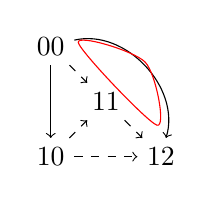
\begin{tikzpicture}
            \node (A) at (-0.7,0.7) {$00$};
            \node (B) at (-0.7,-0.7) {$10$};
            \node (C) at (0.7,-0.7) {$12$};
            \node (D) at (0,0) {$11$};
            \draw [-> ] (A) -- (B);
            \draw[->] (A) to [bend left=60] (C);
            \draw [->, dashed] (A) -- (D);
            \draw [->, dashed] (B) -- (C);
            \draw [->, dashed] (B) -- (D);
            \draw [->, dashed] (D) -- (C);
            \draw [red] [smooth cycle] plot coordinates { (-0.35,0.75) (0.65,-0.3) (0.5,0.5)};
        \end{tikzpicture}
    \ar[r]
    \ar[d, hook]
    &
        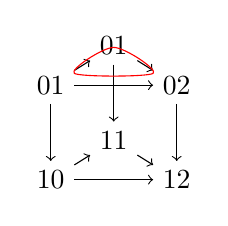
\begin{tikzpicture}
            \node (A) at (0, 0.85) {$01$};
            \node (B) at (-0.8, 0.35) {$01$};
            \node (C) at (0.8, 0.35) {$02$};
            \node (D) at (0, -0.35) {$11$};
            \node (E) at (-0.8, -0.85) {$10$};
            \node (F) at (0.8, -0.85) {$12$};
            \draw[->] (A) to (C);
            \draw[->] (A) to (D);
            \draw[->] (B) to (C);
            \draw[->] (B) to (A);
            \draw[->] (B) to (E);
            \draw[->] (C) to (F);
            \draw[->] (D) to (F);
            \draw[->] (E) to (F);
            \draw[->] (E) to (D);
            \draw [red] [smooth cycle] plot coordinates { (0,0.83) (0.5,0.5) (-0.5,0.5)};
        \end{tikzpicture}
    \ar[d, hook]
    \\
    \Delta^3
    \ar[r, hook, "h_0"']
    &
        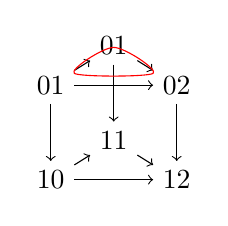
\begin{tikzpicture}
            \node (A) at (0, 0.85) {$01$};
            \node (B) at (-0.8, 0.35) {$01$};
            \node (C) at (0.8, 0.35) {$02$};
            \node (D) at (0, -0.35) {$11$};
            \node (E) at (-0.8, -0.85) {$10$};
            \node (F) at (0.8, -0.85) {$12$};
            \draw[->] (A) to (C);
            \draw[->] (A) to (D);
            \draw[->] (B) to (C);
            \draw[->] (B) to (A);
            \draw[->] (B) to (E);
            \draw[->] (C) to (F);
            \draw[->] (D) to (F);
            \draw[->] (E) to (F);
            \draw[->] (E) to (D);
            \draw [red] [smooth cycle] plot coordinates { (0,0.83) (0.5,0.5) (-0.5,0.5)};
        \end{tikzpicture}
    \end{tikzcd}
    \]
    
    For the case $(\overline{B}_1 \subseteq \overline{B}_2 = \overline{B}_3 )$ we exhibit each horn inclusion $\Lambda_k^n \hookrightarrow \Delta^n$ as a retract of a map in $\overline{B}_3$ for $0 \leq k \leq n$.
    \[
    \begin{tikzcd}
        \Lambda_k^n 
        \ar[r]
        \ar[d, hook]
        \ar[rr, bend left, "\id"]
        &
        (\Delta^1 \times \Lambda_k^n) \cup ( \Delta^{1} \times \Delta^1) 
        \ar[r]
        \ar[d, " \in B_3"]
        &
        \Lambda_k^n
        \ar[d]
        \\
        \Lambda^n 
        \ar[r]
        &
        \Delta^1 \times \Delta^n
        \ar[r]
        &
        \Delta^n
    \end{tikzcd}
    \]
    The vertical maps in the bottom row are given by the following composition of maps of partially ordered sets 
    \[
        [n] \xrightarrow{s} [1] \times [n] \xrightarrow{r} [n]    
    \]
    where the image of $s$ is given as follows
    \[
    s\colon
    \begin{tikzcd}
         01
        \ar[r]
        &
        02
        \ar[r]
        &
        \dotsc
        \ar[r]
        &
        0k
        \ar[rd]
        &
        \\
        &&&&
        1(k+1)
        \ar[r]
        &
        1(k+2)
        \ar[r]
        &
        \dotsc
        \ar[r]
        &
        1n
    \end{tikzcd}
    \]
    and the image of the map $r$ is given by
    \[
    r\colon
    \begin{tikzcd}
        0
        \ar[r]
        \ar[d]
        &
        1
        \ar[r]
        \ar[d]
        &
        2
        \ar[r]
        \ar[d]
        &
        \dotsc
        \ar[r]
        &
        k-1
        \ar[r]
        \ar[d]
        &
        k
        \ar[r]
        \ar[d]
        &
        \dotsc
        \ar[r]
        &
        k
        \ar[d]
        \\
        k
        \ar[r]
        &
        k
        \ar[r]
        &
        k
        \ar[r]
        &
        \dotsc
        \ar[r]
        &
        k
        \ar[r]
        &
        k+1
        \ar[r]
        &
        \dotsc
        \ar[r]
        &
        n
    \end{tikzcd}
    \]
\end{proof}

\begin{cor}
    Let $ S \xhookrightarrow{\iota} T$ be an anodyne extension and $L \xhookrightarrow{i}  K$ be an arbitrary inclusion.
    Then 
    \[
        (S \times K) \cup (T \times L) \xrightarrow{incl.} T \times K
    \]
    is an anodyne extension.
    In particular for $S= \Lambda_k^n$ and $T=\Delta^n$ we obtain that 
    \[
        (\Lambda_k^n \times K) \cup (\Delta^n \times L) \xrightarrow{incl.} \Delta^n \times K
    \]
    is an anodyne extension.
\end{cor}

\begin{proof}
    For 
    $ L \xrightarrow{i} K$ define $\mathcal{M} \coloneqq \{ S \xhookrightarrow{i} T \mid (S \times K) \cup (T \times L) \xrightarrow{} T \times K \text{ is anodyne}\}$
    Notice that $\mathcal{M}$ is a saturated class 
    hence if $\mathcal{M} \supseteq B_3 \implies \mathcal{M} = \overline{B}_3$.
    Consider $L' \hookrightarrow K'$ a monomorphism, that gives rise to $S = ( \Delta^1 \times L') \cup ( \Delta^{\{l\}} \times K') \to \Delta^1 \times K'= T$
    
    \[
    \begin{tikzcd}
        (((\Delta^1 \times L') \cup ( \Delta^{\{l\}} \times K')) \times K ) 
        \ar[r, " \in \An"]
        \ar[d, "\cong"]
        &
        (\Delta^1 \times K') \times K 
        \ar[d,"\cong"]
        \\
        \Delta^1 \times ( L' \times K \cup K' \times L) \cup ( \Delta^{\{l\}} \times (K' \times K) )
        \ar[r]
        &
        \Delta^1 \times (K' \times K)
    \end{tikzcd}
    \]
    Where the vertical map in the top row is in $B_3$ and thus an anodyne extension.
    It follows the bottom row is an anodyne extension as well, which we wanted to show.
\end{proof}

Let now $X$ be a Kan complex.

\begin{defi}
    Let $x \in X_0$ and $ n \geq 1$. We define 
    \[
    \pi_n(X,x) = \left\{ \Delta^n \xrightarrow{\alpha} X \mid 
    \begin{tikzcd}
        \partial
        \Delta^n
        \ar[r]
        \ar[d, hook]
        &
        \Delta^0
        \ar[d]
        \\
        \Delta^n
        \ar[r]
        &
        X
    \end{tikzcd}
    \right\}
    \big/ \text{htpy relative }\partial\Delta^n 
    \]
\end{defi}

\begin{defi}
\label{simplicial n-sphere}
    The (pointed) simplicial n-sphere is 
    \[
    \begin{tikzcd}
        \partial
        \Delta^n
        \ar[d]
        \ar[r, hook]
        &
        \Delta^n
        \ar[rdd, bend left, "\alpha"]
        \ar[d]
        \\
        \Delta^0
        \ar[r, "x"]
        \ar[drr, bend right, "x"']
        &
        \Delta^n/\partial \Delta^n = S^n
        \ar[rd, "\overline{\alpha}"]       
        \\
        &&
        X
    \end{tikzcd}
    \]
\end{defi}

\begin{prop}
    There are pullback squares $(\partial \Delta^n \xhookrightarrow{i} \Delta^n)$
    \[
    \begin{tikzcd}
        \underline{\Hom}(S^n,X)_x
        \ar[r]
        \ar[d]
        &
        \underline{\Hom}(S^n,X)
        \ar[d, "\ev_*"]
        \ar[r]
        &
        \underline{\Hom}(\Delta^n,X)
        \ar[d,"i^*"]
        \\
        \Delta^0
        \ar[r,"x"]
        \ar[rr, bend right ,"c(x)"']
        &
        X
        \cong 
        \underline{\Hom}(\Delta^0,X)
        \ar[r]
        &
        \underline{\Hom}(\partial \Delta^n,X)
    \end{tikzcd}
    \]
    where the vertical morphisms are Kan Fibrations and $\underline{\Hom}(S^n,X)_x$ is a Kan complex.
    Moreover the induced map 
    \[
        \underline{\Hom}(S^n,X)_x \to \underline{\Hom}(S^n,X)_{c(x)}
    \]
    is an isomorphism (between Kan complexes, since $X$ is a Kan complex).
\end{prop}

\begin{proof}
    Consider the following commutative square
    \[
    \begin{tikzcd}
        \Hom(\Delta^m \times S^n , X ) 
        \ar[r]
        \ar[d]
        &
        \Hom(\Delta^m \times \Delta^n , X )
        \ar[d]
        \\
        \Hom(\Delta^m \times \Delta^0 , X ) 
        \ar[r]
        &
        \Hom(\Delta^m \times \partial \Delta^n , X )
    \end{tikzcd}
    \] 
    this is a pullback since the Hom-functor sends colimits to limits and thus the diagram from \cref{simplicial n-sphere} to a pullback. 
    The left square is a pullback by construction and thus by the Pasting lemma 
    the outer square is a pullback as well.
\end{proof}

Lecture 12.11

\begin{prop}
    Let $X$ be a Kan complex and $x \in X_0$. Then the "old" and "new" definitions of $\pi_1(X,x)$ agree.
\end{prop}

\begin{proof}
    Consider the square
    \[
    \begin{tikzcd}
        \underline{\Hom}(\Delta^1, X)_{c(x)} 
        \ar[r]
        \ar[d]
        &
        \underline{\Hom}(\Delta^1, X)
        \ar[d, "i_*"]
        \\
        \Delta^0
        \ar[r, "{c(x)=(x,x)}"]
        &
        \underline{\Hom}(\partial \Delta^1, X) \cong X \times X
    \end{tikzcd}
    \]
    and let $f,g\colon \Delta^1 \to X$ such that $f_{\mid \partial \Delta^1}=(x,x)=g_{\mid \partial \Delta^1}$. 
    A homotopy $h\colon f \to g$ (rel $\partial \Delta^1$) is by definition 
    \[
    \begin{tikzcd}
        \Delta^{0}\times \Delta^{1}
        \ar[d]
        \ar[rd, bend left, "f"]
        &
        \\
        \Delta^1 \times \Delta^1
        \ar[r, "h"]
        &
        X
        \\
        \Delta^{1} \times \Delta^1
        \ar[u]
        \ar[ru, bend right, "g"']
    \end{tikzcd}
    \]
    the homotopy yields the following commutative square 
    \[
    \begin{tikzcd}
        x 
        \ar[r, "f"]
        \ar[d, equal]
        \ar[rd, "u"]
        &
        x
        \ar[d, equal]
        \\
        x
        \ar[r, "g"']
        &
        x
    \end{tikzcd}
    \]
\end{proof}

\underline{Aim}: To prove that $\pi_n(X,x)$ is a group for $n \geq 1$ (that is abelian for $n \geq 2$) as well as functoriality.
Fix $(X,x)$ where $X$ is a Kan complex $x \in X_0$, take n-simplices $\alpha, \beta  \colon  \Delta^n \to X$ representatives of classes in $\pi_n(X,x)$ that is $\alpha_{\mid \partial \Delta^n}= c(x) = \beta_{\mid \partial \Delta^n}$.
For $n=1$ this yields a horn, which can be extended since $X$ is a Kan complex. 
\[
\begin{tikzcd}
    &
    x
    \ar[rd, "\beta"]
    &
    \\
    x
    \ar[ru, "\alpha"]
    \ar[rr, dashed, "\gamma"']
    &&
    x
\end{tikzcd}
\]
For the general case we obtain a map from the horn (given on its n-simplices) as follows 
\[
\begin{tikzcd}
    \Lambda_n^{(n+1)}
    \ar[rr,"{(x,x,\dotsc,x,\alpha,\bullet,\beta)}"]
    \ar[d, hook]
    &&
    X
    \\
    \Delta^{(n+1)}
    \ar[rru, dashed, "\exists \sigma"']
    &&
\end{tikzcd}
\]
where $d_n\sigma\eqqcolon \gamma$ is the composition of $\alpha$ and $\beta$.
Now we define the multiplicative law on $\pi_n(X,x)$ by 
\begin{align*}
    \pi_n(X,x) \times \pi_n(X,x)& \to \pi_n(X,x)\\
    ([\alpha],[\beta])& \mapsto[\gamma]
\end{align*}

\begin{prop}
    The above binary operation is well defined.
\end{prop}

\begin{proof}
    We have $\alpha,\alpha',\beta,\beta'\colon \Delta^n \to X$ are representatives in $\pi_n(X,x)$ and
    \begin{align*}
        h_{n-1} \colon \Delta^1\times \Delta^n \to X \text{ htpy } \alpha \to \alpha' (\rel \partial \Delta^n)\\
        h_{n-1} \colon \Delta^1\times \Delta^n \to X \text{ htpy } \beta \to \beta' (\rel \partial \Delta^n)
    \end{align*}
    Choose $w,w' \colon \Delta^{n+1} \to X$ such that 
    \begin{align*}
        &\partial w = (x, \dotsc, x, \alpha, \gamma, \beta)\\
        &\partial w' = (x, \dotsc, x, \alpha', \gamma', \beta')
    \end{align*}
    Putting all this together we obtain 
    \[
    \begin{tikzcd}
        (\Delta^{(n+1)} \times \partial \Delta^1) \cup (\Delta^1 \times \Lambda_n^{n+1})
        \ar[rrr, "{(w,w',(x, \dotsc , x , h_{n-1}, \bullet, h_{n})}"]
        \ar[d, hook]
        &&&
        X
        \\
        \Delta^1 \times \Delta^{(n+1)}
        \ar[rrru, "w''"']
        &&
    \end{tikzcd}
    \]
    where $w''$ exists, since on the one summand we just have an inclusion and on the other we use that $X$ is a Kan complex.
    This way the composite
    \[
    h_n \colon \Delta^1 \times \Delta^n \xrightarrow{1 \times d^n} \Delta^1 \times \Delta^{n+1} \xrightarrow{w''} X
    \]
    is a homotopy from $\gamma$ to $\gamma'$ ($\rel \partial \Delta^n)$.
\end{proof}
Let us take a look at the case $n=1$ explicitely.
    
\[
    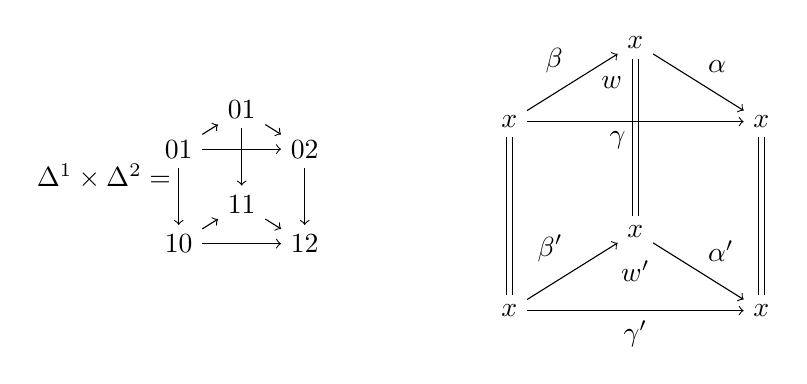
\begin{tikzpicture}
    \begin{scope}
        \node (0) at (-1.75,0) {$\Delta^1 \times \Delta^2 =$};
        \node (A) at (0, 0.85) {$01$};
        \node (B) at (-0.8, 0.35) {$01$};
        \node (C) at (0.8, 0.35) {$02$};
        \node (D) at (0, -0.35) {$11$};
        \node (E) at (-0.8, -0.85) {$10$};
        \node (F) at (0.8, -0.85) {$12$};
        \draw[->] (A) to (C);
        \draw[->] (A) to (D);
        \draw[->] (B) to (C);
        \draw[->] (B) to (A);
        \draw[->] (B) to (E);
        \draw[->] (C) to (F);
        \draw[->] (D) to (F);
        \draw[->] (E) to (F);
        \draw[->] (E) to (D);
    \end{scope}

    \begin{scope}[xshift=5cm]
        \node(arrow) at ( -3,0) {$\rightsquigarrow$};
        \node (A) at (0, 1.7) {$x$};
        \node (w) at (-0.3, 1.2) {$w$};
        \node (B) at (-1.6, 0.7) {$x$};
        \node (C) at (1.6, 0.7) {$x$};
        \node (D) at (0, -0.7) {$x$};
        \node (w') at (0, -1.2) {$w'$};
        \node (E) at (-1.6, -1.7) {$x$};
        \node (F) at (1.6, -1.7) {$x$};
        \draw[->] (A) to node[above right ]{$\alpha$} (C) ;
        \draw[double equal sign distance] (A) to (D) ;
        \draw[->] (B) to node[below left]{$\gamma$} (C);
        \draw[->] (B) to node[above left]{$\beta$} (A);
        \draw[double equal sign distance] (B) to (E) ;
        \draw[double equal sign distance] (C) to (F);
        \draw[->] (D) to node[above right ]{$\alpha'$} (F);
        \draw[->] (E) to node[below]{$\gamma'$} (F);
        \draw[->] (E) to node[above left]{$\beta'$} (D);
    \end{scope}
    \end{tikzpicture}
\]
\begin{prop}
    For all $n \geq 1$ it holds that $ \pi_n(X,x)$ is a group.
\end{prop}

\begin{proof}
    (Unitality) The neutral element in $\pi_n(X,x)$ is given by $[c(x)]$, where 
    \[
    c^n(x)\colon 
    \begin{tikzcd}
        &
        \Delta^0
        \ar[rd, "x"]
        &
        \\
        \Delta^n
        \ar[ru]
        \ar[rr]
        &&
        X
    \end{tikzcd}
    \]
    Let $w\coloneqq s_n(\alpha) \colon \Delta^{n+1} \to X$ for $\alpha\colon \Delta^n \to X$ such that $d_{n+1}(w)=d_{n+1}(s_n(\alpha))=\alpha=d_n(s_n(\alpha))=d_n(w)$.
    \[
    \begin{tikzcd}
        \Lambda_k^{n+1}
        \ar[d, hook]
        \ar[rrr, "{(x,x,\dotsc,x,c^n(x), \bullet, \alpha)}"]
        &&&
        X
        \\
        \Delta^{n+1}
        \ar[rrru, "w"']
    \end{tikzcd}
    \]
    where $[c^n(x)][\alpha]=[\alpha]$.

    (Associativity)
    Let $\alpha, \beta, \gamma \colon \Delta^n \to X$ be representatives of classes in $\pi_n(X,x)$.
    Choose $w_{n-1},w_{n+1},w_{n+2}\colon \Delta^{n+1} \to X$ such that 
    \begin{align*}
        \partial w_{n-1} =(x, \dotsc, x, \alpha, u, \beta) &; [\alpha][\beta]=[u]\\
        \partial w_{n+1} =(x, \dotsc, x, u, v, \gamma) &; [u][\gamma]=[v]\\
        \partial w_{n+2} =(x, \dotsc, x, \beta, \omega, \gamma) &; [\beta][\gamma]=[\omega]
    \end{align*}
    Let $q=(c^{n+1}(x), \dotsc , c^{n+1}(x), w_{n-1}, \bullet, w_{n+1}, w_{n+2})$, we obtain a diagram
    \[
    \begin{tikzcd}
        \Lambda_n^{n+2}
        \ar[r, "q"]
        \ar[d, hook]
        &
        X
        \\
        \Delta^{n+2}
        \ar[ru, " \exists \Tilde{w}"']
    \end{tikzcd}
    \]
    Now let us define $w_n \coloneqq d_n(\Tilde{w})$ and thus $\partial w_n = (x, \dotsc , x , \alpha, v, \omega) ; [\alpha][\omega]=[v]$. This results in 
    \[
    ([\alpha][\beta])[\gamma]=[u][\gamma]=[v]=[\alpha][w]=[\alpha]([\beta][\gamma])
    \]
    
    (Inverses)
    Let $\Delta^n \xrightarrow{\alpha} X$ be a representative of a calass in $\pi_n(X,x)$. 
    Consider the following horn-extension diagram
    \[
    \begin{tikzcd}
        \Lambda_n^{n+1}
        \ar[rrr, "{(x, \dotsc , x , \bullet , c^n(x), \alpha)}"]
        \arrow[d, hook]
        &&&
        X
        \\
        \Delta^{n+2}
        \ar[rrru, " \exists w"]
    \end{tikzcd}
    \]
    thus we get the equation $[d_{n-1}(w)][\alpha]=[c^n(x)]$

\underline{Aim}: Establish the functoriality of $\pi_n(X,x)$ and let $(X,x)$ and $(Y,y)$ be pairs such that $Y,X$ are Kan complexes $x \in X_0$ and $y \in Y_0$ and $f\colon X \to Y$ such that $f_0(x)=y$.
\[
    \begin{tikzcd}
        \underline{\Hom}(\Delta^n,X)_{c^n(x)}
        \ar[dd]
        \ar[rr]
        \ar[rd, "f_*"]
        &&
        \underline{\Hom}(\Delta^n,X)
        %\ar[d, "{\iota_*}"]
        \ar[rd, "f_*"]
        &
        \\
        &
        \underline{\Hom}(\Delta^n,Y)_{c^n(y)}
        \ar[dd]
        \ar[rr]
        &&
        \Hom(\Delta^n,Y)
        \ar[dd]
        \\
        \Delta^0
        \ar[rd, equal]
        \ar[rr, "c^n(x)"]
        &&
        \underline{\Hom(\partial \Delta^n,X)}
        \ar[rd, "f^*"]
        &
        \\
        &
        \Delta^0
        \ar[rr, "c^n(y)"]
        &&
        \underline{\Hom(\partial \Delta^n, X)}
    \end{tikzcd}
\]
For $i \colon \partial \Delta^n \to \Delta^n$.
Then $\pi_0(f_*) \eqqcolon \pi_n(f) \colon \pi_n(X,x) \to \pi_n(Y,y)$ is a morphism of pointed sets and gives the functoriality.
\end{proof}

\begin{defi}
    Let $\Delta^0/\SetD$ be the category of pointed sets.
\end{defi}

\begin{prop}
    Let $f\colon (X,x) \to (Y,y)$ be a morphism of pointed Kan complexes, then 
    \[
    \pi_n(f) \colon \pi_n(X,x) \to \pi_n(Y,y) 
    \]
    is a group homomorphism.
\end{prop}

\begin{proof}
    Let $\alpha, \beta \colon \Delta^n \to X$ be representatives of classes in $\pi_n(X,x)$ and
    $w \colon \Delta^{n+1} \to X$ where $\partial w = (x, \dotsc ,x , \alpha, \gamma , \beta)$ so that 
    $[\alpha][\beta]=[\gamma]$. But then
    \[
    f_*(w)\colon \Delta^{n+1}\xrightarrow{w}X \xrightarrow{f}Y
    \]
    has boundary $\partial (f_*(w))=(y, \dotsc , y, f_*(\alpha),f_*(\gamma),f_*(\beta))$
\end{proof}

\begin{prop}
    Let $f_1, f_2 \colon X \to Y$ and $g_1, g_2 \colon Y \to Z$ be morphisms between Kan complexes.
    Supose that $f_1 \sim f_2$ and $g_1 \sim g_2$, then $ g_1 \circ f_1 \sim g_2 \circ f_2$
\end{prop}

\begin{proof}
    Enough to treat the case $(f_1 = f_2, g_1 \sim g_2)$ and $(f_1 \sim f_2, g_1 = g_2)$.
    The first case is $f\coloneqq f_1 = f_2$ and $g_1 \sim g_2$, which gives 
    \[
    \begin{tikzcd}
        X  \cong \Delta^{\{0\}} \times X 
        \ar[r, "\id \times f"]
        \ar[d, "i_0 \times \id"']
        &
        \Delta^{\{0\}} \times Y
        \ar[d]
        \ar[rd, bend left, "g_1"]
        &
        \\
        \Delta^1 \times X
        \ar[r, "\id \times f"]
        &
        \Delta^1 \times X
        \ar[r, "h"]
        &
        Z
        \\
        X \cong \Delta^{\{1\}} \times X
        \ar[u, "i_1 \times \id"]
        \ar[r, "\id \times f"]
        &
        \Delta^{\{1\}}\times Y
        \ar[u]
        \ar[ru, bend right, "g_2"']
    \end{tikzcd}
    \]
    $h_f \colon g_1f \to g_2f$ is a homotopy of of the concatenation.

    The second case is $g\coloneqq g_1 = g_2$
    \[
    \begin{tikzcd}
        \Delta^{\{0\}}\times X
        \ar[d]
        \ar[dr, bend left, "f_1"]
        \ar[drr, bend left, "gf_1"]
        \\
        \Delta^1 \times X 
        \ar[r, "h"]
        &
        Y
        \ar[r]
        &
        Z
        \\
        \Delta^{\{1\}} \times X
        \ar[u]
        \ar[ru,bend right, "f_2"']
        \ar[rru,bend right, "gf_2"']
    \end{tikzcd}
    \]
    The horizontal composition then gives a homotopy from $gf_1$ to $gf_2$.
\end{proof}

\subsection{Exercises}

\begin{Exercise}
    
Consider a set $ G $ with two unital binary operations $ \otimes : G \times G \to G $.
Suppose that 
\[
    ( a \otimes b ) \cdot ( c \otimes d ) = ( a \cdot c ) \otimes ( b \cdot d )
\]
for all $ a , b, c , d \in G $.
\begin{enumerate}
    \item 
    Show that both units $e$ and $e_{\otimes}$ agree.

    \item 
    Deduce that $ \cdot = \otimes $.

    \item 
    Conclude that $ ( G , \cdot , e ) $ is an abelian monoid.
\end{enumerate}
\end{Exercise}


\begin{Exercise}
\label{Exercise_11.2}

Fix a Kan complex $ X $ and $ n \in \mathbb{N}_0$.

\begin{enumerate}[label=(\alph*)]
    \item 
    Let $ \alpha: \Delta^n \to X $ represent an element of $ \pi_n ( X , x ) $ for some $ x \in X_0 $ and $ n \in \mathbb{N}_0 $.
    Show that $ \alpha $ is homotopic to the neutral element $ x : \Delta^n \to \Delta^0 \xrightarrow{x} X $ if and only if there exists some $ \sigma \in \Delta^{n+1}$ such that $ d_i ( \sigma ) = x $ for $ 0 \leq  i \leq n $ and $ d_{n+1} ( \sigma ) = \alpha $.

    \item 
    Deduce that if $ p : X \to \Delta^0 $ is a trivial Kan fibration, i.e. $p \in r ( \{ \partial \Delta^n \to \Delta^n \mid n \in \mathbb{N}_0 \} )$, then $ \pi_n( X , x ) = 0 $ for all $ x \in X_0 $.

    \item 
    Deduce that for $X$ $n$-skeletal we have that $\pi_m ( X , x ) \cong 0 $ for any $ x \in X_0 $ and $ m \geq n $.

    \item 
    Show that for a group $ G $ we have that 
    \[
        \pi_n ( N ( BG ) , \star ) 
        \cong 
        \begin{cases}
            G &\text{ if }  n = 1
            \\
            0 &\text{ if }  n \neq 1
        \end{cases}
    \]
    where $ \star $ is the unique object of $ BG $.
\end{enumerate}
\end{Exercise}



